\documentclass{article}
\usepackage[a4paper,left=3cm, right=3cm, top=2cm, bottom=2cm]{geometry}
\usepackage{amsmath}
\usepackage{graphicx}
\usepackage{caption}
\usepackage{setspace}
\usepackage{xcolor}
\usepackage{titlesec}
\usepackage{amssymb}
\usepackage{tcolorbox}
\usepackage{wrapfig}
\usepackage{amsthm} % For proofs

\graphicspath{{graph/}}
\title{11.9 Representations of Functions as Power Series}
\date{}
\author{}
\setstretch{1.3}

% \subsection* 형식 지정 (번호 없음)
\titleformat{name=\section, numberless}
  {\normalfont\large\bfseries\color{blue}}
  {}
  {0pt}
  {}
\geometry{a4paper, margin=1in}

% 증명 환경 스타일
\newtheoremstyle{mystyle}% name
  {}% Space above
  {}% Space below
  {\itshape}% Body font
  {}% Indent amount
  {\bfseries}% Theorem head font
  {.}% Punctuation after theorem head
  {.5em}% Space after theorem head
  {}% Theorem head spec (can be left empty, meaning `normal')
\theoremstyle{mystyle}

\begin{document}
\maketitle

In this section we learn how to represent certain types of functions as sums of power series by manipulating geometric series or by differentiating or integrating such a series. This is useful because representing a function as a power series gives us a way to approximate the function with polynomials.


We start with the geometric series equation:
\begin{equation*}
    \frac{1}{1-x} = 1 + x + x^2 + x^3 + \cdots = \sum_{n=0}^{\infty} x^n \quad |x| < 1 \label{eq:geom_series}
\end{equation*}

A geometric illustration is shown in picture. Because the sum of a series is the limit of the sequence of partial sums, we have
    \[\frac{1}{1-x} = \lim_{n\to\infty} s_n(x)\]
    \[s_n(x) = 1+x+x^2+...+x^n\]

\begin{figure}[htbp]

    \centering
    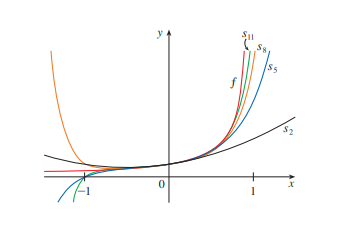
\includegraphics[width=0.5\textwidth]{graph 78.png}
\end{figure}

\subsection*{EXAMPLE 1}
Express \( \dfrac{1}{1+x^2} \) as the sum of a power series and find the radius of convergence.\\
\textbf{SOLUTION:}
Replacing \(x\) by \(-x^2\) in Equation (\ref{eq:geom_series}), we have
\begin{align*}
    \dfrac{1}{1+x^2} = \dfrac{1}{1-(-x^2)} &= \sum_{n=0}^{\infty} (-x^2)^n \\
    &= \sum_{n=0}^{\infty} (-1)^n x^{2n} = 1 - x^2 + x^4 - x^6 + x^8 - \cdots
\end{align*}
Because this is a geometric series, it converges when \(|-x^2| < 1\), that is, \(x^2 < 1\), or \(|x| < 1\). Therefore the radius of convergence is \(R=1\).

\subsection*{EXAMPLE 2}
Find a power series representation for \( \dfrac{1}{x+2} \).\\
\textbf{SOLUTION:}
We first rewrite the function in the form \(1/(1-r)\):
\[ \dfrac{1}{2+x} = \dfrac{1}{2(1 + x/2)} = \dfrac{1}{2[1 - (-x/2)]} = \dfrac{1}{2} \sum_{n=0}^{\infty} \left(-\dfrac{x}{2}\right)^n \]
This series converges when \(|-x/2| < 1\), that is, \(|x| < 2\). So the radius of convergence is \(R=2\). The power series representation is:
\[ \dfrac{1}{x+2} = \dfrac{1}{2} \sum_{n=0}^{\infty} \dfrac{(-1)^n}{2^n} x^n = \sum_{n=0}^{\infty} \dfrac{(-1)^n}{2^{n+1}} x^n \]

\subsection*{EXAMPLE 3}
Find a power series representation of \( \dfrac{x^3}{x+2} \).\\
\textbf{SOLUTION:}
Since this function is just \(x^3\) times the function in Example 2, all we have to do is multiply that series by \(x^3\):
\begin{align*}
    \dfrac{x^3}{x+2} &= x^3 \sum_{n=0}^{\infty} \dfrac{(-1)^n}{2^{n+1}} x^n = \sum_{n=0}^{\infty} \dfrac{(-1)^n}{2^{n+1}} x^{n+3} \\
    &= \dfrac{1}{2}x^3 - \dfrac{1}{4}x^4 + \dfrac{1}{8}x^5 - \dfrac{1}{16}x^6 + \cdots
\end{align*}
This series converges for \(|x|<2\).

\section*{Differentiation and Integration of Power Series}
The sum of a power series is a function \(f(x) = \sum_{n=0}^\infty c_n (x-a)^n\) whose domain is the interval of convergence. We can differentiate and integrate such functions term by term.

\begin{tcolorbox}[
    colback=white,
    colframe=orange!80!white,
    title=Theorem 1: Term-by-Term Differentiation and Integration,
    boxrule=0.5mm,
    arc=3mm
    ]
    If the power series \( \sum c_n (x-a)^n \) has radius of convergence \(R > 0\), then the function \(f\) defined by
    \[ f(x) = c_0 + c_1(x-a) + c_2(x-a)^2 + \cdots = \sum_{n=0}^{\infty} c_n (x-a)^n \]
    is differentiable (and therefore continuous) on the interval \((a-R, a+R)\) and
    \begin{itemize}
        \item[(i)] \( f'(x) = c_1 + 2c_2(x-a) + 3c_3(x-a)^2 + \cdots = \sum_{n=1}^{\infty} n c_n (x-a)^{n-1} \)
        \item[(ii)] \( \int f(x) \,dx = C + c_0(x-a) + c_1\dfrac{(x-a)^2}{2} + c_2\dfrac{(x-a)^3}{3} + \cdots = C + \sum_{n=0}^{\infty} c_n \dfrac{(x-a)^{n+1}}{n+1} \)
    \end{itemize}
    The radii of convergence of the power series in Equations (i) and (ii) are both \(R\).
   \\ \textbf{Note:} The interval of convergence may change at the endpoints after differentiation or integration.
\end{tcolorbox}

\subsection*{EXAMPLE 4}
Express $\dfrac{1}{(1-x)^2}$ as a power series by differentiating $\dfrac{1}{(1-x)}$. What is the radius of convergence?\\
\textbf{SOLUTION:}
We start with 
\[\dfrac{1}{1-x} = 1 + x + x^2 + x^3 + \cdots = \sum_{n=0}^{\infty} x^n\]
Differenrialting both sides term by term, we get
\[\dfrac{1}{(1-x)^2} = 1 + 2x + 3x^2 + 4x^3 + \cdots = \sum_{n=1}^{\infty} nx^{n-1}=\sum_{n=0}^{\infty} (n+1)x^n\]
According to Theorem 2, the radius of convergence of the differentiated series is the same as the radius of convergence of the original series, \(R=1\).

\subsection*{EXAMPLE 5}
Find a power series representation for \( \ln(1+x) \) and its radius of convergence.\\
\textbf{SOLUTION:}
We notice that, except for a factor of \(-1\), the derivative of \(\ln(1+x)\) is \(1/(1-x)\).
\[ \ln(1+x) = \int \dfrac{1}{1+x} \,dx = \int (1 - x + x^2 -\cdots) \,dx = x - \dfrac{x^2}{2} + \dfrac{x^3}{3} - \cdots + C = \sum_{n=0}^{\infty} (-1)^{n}\dfrac{x^{n+1}}{n+1} + C \]
Letting \(x=0\), we get \(\ln(1) = 0+C\), so \(C=0\). Thus
\[ \ln(1+x) = \sum_{n=1}^{\infty} (-1)^{n-1}\dfrac{x^{n}}{n} \]

The radius of convergence is the same as the original series, \(R=1\).

\subsection*{EXAMPLE 6}
Find a power series representation for \(f(x) = \tan^{-1}(x)\).\\
\textbf{SOLUTION:}
We observe that \(f'(x) = \dfrac{1}{1+x^2}\). From Example 1, we have
\[ \dfrac{1}{1+x^2} = \sum_{n=0}^{\infty} (-1)^n x^{2n} \quad (|x|<1) \]
Integrating term by term, we get
\begin{align*}
    \tan^{-1}(x) &= \int \dfrac{1}{1+x^2} \,dx = \int \left( \sum_{n=0}^{\infty} (-1)^n x^{2n} \right) \,dx \\
    &= C + \sum_{n=0}^{\infty} (-1)^n \dfrac{x^{2n+1}}{2n+1}
\end{align*}
To find \(C\), we put \(x=0\). Then \(C = \tan^{-1}(0) = 0\). Therefore
\[ \tan^{-1}(x) = \sum_{n=0}^{\infty} (-1)^n \dfrac{x^{2n+1}}{2n+1} = x - \dfrac{x^3}{3} + \dfrac{x^5}{5} - \dfrac{x^7}{7} + \cdots \]
The radius of convergence is \(R=1\).

\subsection*{EXAMPLE 7}
(a) Evaluate \( \int \dfrac{1}{1+x^7} \,dx \) as a power series. \\
(b) Use part (a) to approximate \( \int_0^{0.5} \dfrac{1}{1+x^7} \,dx \) correct to six decimal places.\\
\textbf{SOLUTION:}
\begin{itemize}
    \item[(a)] Replacing \(x\) with \(x^7\) in Equation (\ref{eq:geom_series}), we get
    \[ \dfrac{1}{1+x^7} = \dfrac{1}{1-(-x^7)} = \sum_{n=0}^{\infty} (-x^7)^n = \sum_{n=0}^{\infty} (-1)^n x^{7n} \quad (|x|<1) \]
    Integrating term by term:
    \[ \int \dfrac{1}{1+x^7} \,dx = \int \sum_{n=0}^{\infty} (-1)^n x^{7n} \,dx = C + \sum_{n=0}^{\infty} (-1)^n \dfrac{x^{7n+1}}{7n+1} \]
    The radius of convergence is \(R=1\).
    \item[(b)] Using the result from part (a):
    \[ \int_0^{0.5} \dfrac{1}{1+x^7} \,dx = \left[ x - \dfrac{x^8}{8} + \dfrac{x^{15}}{15} - \dfrac{x^{22}}{22} + \cdots \right]_0^{0.5} \]
    \[ = 0.5 - \dfrac{(0.5)^8}{8} + \dfrac{(0.5)^{15}}{15} - \dfrac{(0.5)^{22}}{22} + \cdots \]
    This is an alternating series. The terms are:
    \begin{align*}
        b_0 &= 0.5 \\
        b_1 &= \dfrac{(0.5)^8}{8} \approx 0.00048828 \\
        b_2 &= \dfrac{(0.5)^{15}}{15} \approx 0.00000203 \\
        b_3 &= \dfrac{(0.5)^{22}}{22} \approx 0.00000001
    \end{align*}
    By the Alternating Series Estimation Theorem, the error is less than \(b_3\). To ensure six decimal place accuracy, we need the error to be less than \(0.0000005\). Since \(b_3 < 0.0000005\), we can use the sum up to \(b_2\):
    \[ \int_0^{0.5} \dfrac{1}{1+x^7} \,dx \approx 0.5 - \dfrac{(0.5)^8}{8} + \dfrac{(0.5)^{15}}{15} \approx 0.5 - 0.00048828 + 0.00000203 \approx 0.49951375 \]
    Rounding to six decimal places, we get \(0.499514\).
\end{itemize}

\end{document}